\documentclass[12pt, a4paper]{article}

\usepackage[utf8]{inputenc}
\usepackage[russian]{babel}
\parindent 0pt
\parskip 8pt
\usepackage{amsmath}
\usepackage{amssymb}
\usepackage{array}
\usepackage{floatrow}
\usepackage{float}
\usepackage[left=2.3cm, right=2.3cm, top=2.7cm, bottom=2.7cm, bindingoffset=0cm]{geometry} % headheight=0pt,
\usepackage{hyperref}
\usepackage{graphicx}
\usepackage{multicol}
\usepackage{fancyhdr} 
\usepackage{extramarks}
\usepackage[usenames,dvipsnames]{color}
\usepackage{titlesec}
\usepackage{tikz}
\definecolor{grey}{RGB}{128,128,128}

\pagestyle{fancy}
\fancyhf{}
\lhead{Билет № 2.3-4}
\chead{Конвейерная архитектура. Конвейер MIPS. Конфликты конвеера}
\rhead{\thepage}
\lfoot{made with Ы}
\cfoot{}
\rfoot{\today}
\renewcommand\headrulewidth{0.4pt}
\renewcommand\footrulewidth{0.4pt}

\titlespacing*{\section}{0pt}{5pt}{0pt}
\titlespacing*{\subsection}{0pt}{5pt}{0pt}
\titlespacing*{\subsubsection}{0pt}{5pt}{0pt}

\begin{document}
\section{Конвеер}
Заметим, что если выполнять все инструкции на железке последовательно, то во время выполнения каждой инструкции много железа будет просто не использоваться.\\
Давайте разделим процесс выполнения на несколько независимых стадий. И будем выполнять каждую за один такт. Собственно, когда первая команда перешла на вторую стадию выполнения, на первую уже можно подать следующую команду и так далее.
\section{Конвеер MIPS}
\begin{figure}[h]
    \centering
    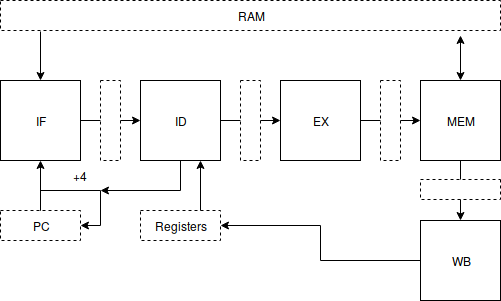
\includegraphics[width = 0.8\linewidth]{./images/MIPS.png}
    \caption{MIPS конвеер}
    \label{fig:MIPS}
\end{figure}
Стадии:
\begin{itemize}
    \item Instruction Fetch
    \item Instruction Decode
    \item Execute
    \item MEM
    \item Write-back
\end{itemize}
\begin{figure}[h]
    \centering
    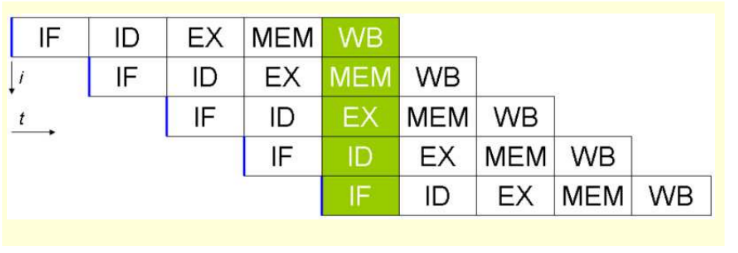
\includegraphics[width=0.8\linewidth]{./images/pipe.png}
    \label{fig:pipe}
\end{figure}
\subsection{Instruction Fetch}
На этой стадии выполняется чтение команды из памяти.\\
У CPU есть специальный регистр, \textbf{PC} (Program Counter в MIPS, в x86 он называется IP - Instruction Pointer), в нем хранится адрес выполняемой команды.\\
На этой стадии из памяти считывается четыре байта (размер одной команды в MIPS), затем счетчик PC увеличивается на четыре.
\subsection{Instruction Decode}
На этой стадии команда декодируется. Т.е. разбираем команду на:
\begin{itemize}
    \item код операции
    \item коды регистров-операндов
    \item код константы (если есть)
\end{itemize}
Если в команде фигурировали значения регистров, то мы считываем эти значения во второй половине такта (на спаде импульса синхронизации).
\subsection{Execute}
На этой стадии выполняются операции с операндами (которые декодировали на предыдущей стадии). Для операций LD и ST на этой стадии считается адрес.
\subsection{MEM}
На этой стадии происходит чтение/запись в память. 
\subsection{Write-Back}
На этой стадии (в первой половине такта, по фронту имульса синхронизации) всё, что было посчитано или считано из памяти пишется в регистры.
\section{Почему это быстрее?}
Во-первых, так как стадии простые, выполняются они быстрее. Следовательно можно увеличить тактовую частоту.\\
Во-вторых, не смотря на то, что у нас могла увеличиться lattency (м.б. раньше мы делали одну команду за 2 такта, а теперь делаем её за 5), у нас сильно увеличилсь throughput (новые команды получаем каждый такт). Одна команда выполнится за 5 тактов, а сто команд - за 104 такта (в среднем каждая команда выполнится за 1 такт, ничего так).\\
Скорость работы $= Clock * IPC$\\
\textbf{IPC} - Instruction Per Clock - сколько полезного делаем за один такт. На конвеере мы увеличиваем оба параметра, поэтому скорость растёт.
\section{Примеры}
ADD R0 R1 5
\begin{enumerate}
    \item IF: Из памяти считана инструкция. PC += 4
    \item ID: Инструкция декодирована. Команда: ADD, Операнды: regs[R1], 5. Записано должно быть в R0.
    \item EX: Выполнено сложение.
    \item MEM: NOP. Эта команда не обращается к памяти, на этой стадии с ней ничего не происходит.
    \item WB: Результат сложения пишется в регистр R0.
\end{enumerate}
\section{Конфликты конвеера}
\subsection{Data hazard}
Data hazards - конфликты, возникающие из-за того, что инструкции не независимы.\\
Пример:\\
ADD R1 R2 R3\\
SUB R4 R5 R1\\
XOR ...
\begin{figure}[h]
    \centering
    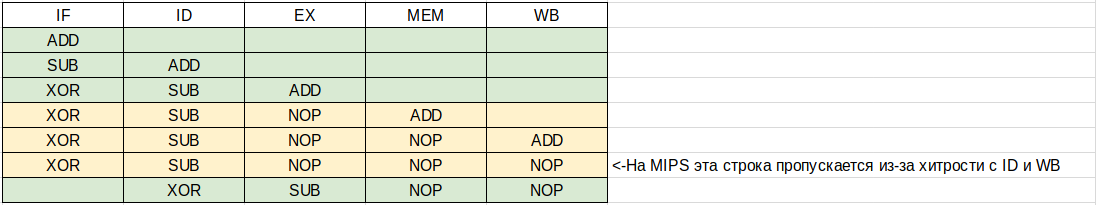
\includegraphics[width = 0.8\linewidth]{./images/RAW.png}
    \caption{Пример RAW хазарда}
    \label{fig:RAW}
\end{figure}\\
Есть несколько подходов к решению такого конфликта:
\begin{enumerate}
    \item Притормозить конвеер, т.е. закинуть на стадии NOP вместо полезных вычислений. В примере можно оставить SUB на стадии ID. Тогда ID отменит изменение PC, а на следующую стадию передаст NOP.
    \item Forwarding. Запросить у одной из следующих стадий уже посчитанное значение. ID может попросить читать значение из следующего буфера.
    \begin{figure}
        \centering
        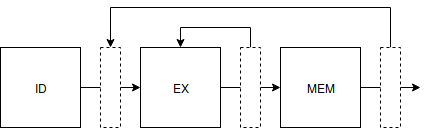
\includegraphics[width=0.8\linewidth]{images/Forwarding.png}
        \caption{Forwarding}
        \label{fig:my_label}
    \end{figure}
    Но если перед SUB была команда загрузки из памяти? Тогда нужна еще одна линия Forwarding. Но команда LD выполняется только на стадии MEM -> на стадию EX всё равно придется кинуть NOP.
    \item Документация. Можно сказать, что то, что команда записывает результат выполнения только через 4 такта - не баг, а фича.
\end{enumerate}
В MIPS конфликты решаются с помощью Forwarding и документации -> там NOP не появляются сами по себе.
\subsection{Control hazards}
Control hazards - конфликты, возникающие из-за инструкций, которые изменяют PC.\\
\textbf{Не рассказывать про branch prediction))0))00}\\
Пример:\\
ADD\\
JMP L1\\
SUB\\
SUB \\
L1: XOR\\
Есть два способа починить:
\begin{enumerate}
    \item Документация
    \item Кидать NOP
\end{enumerate}
Кроме того, обычно JMP исполняется на стадии ID.\\
В MIPS: документация. JMP срабатывает на такт позже -> команда, написанная после команды JMP тоже выполнится. Это место после команды JMP называется "delay slot".
\subsection{Structural hazard}
Structural hazard - конфликты, связанные с нехваткой ресурсов. Т.е. когда железка не может выпонять некоторые команды одновременно на каких-то стадиях.\\
Возникает, например, если у нас один канал к памяти. Если на стадии MEM выполняется LD или ST - не можем считать команду на стадии IF.\\
Как пофиксить:\\
Добавить железа. Либо жить с этим.\\
В MIPS такой проблемы нет, т.к. MIPS - гарвардская архитектура.
\end{document}